\chapter{RELATED WORK}

There have been many research initiatives focusing on occupancy estimation.
Generally speaking, they are based either on images, videos, or RF signals.
Approaches based on camera use captured images to estimate the number of people in a crowded scene~\cite{Ma_2013_CVPR,Pe_count}.
Still, in such camera-based approaches, estimation accuracy can be affected by many factors such as brightness and image resolution.
In addition, camera-based approaches typically lead to high deployment cost.
Other approaches based on RF signals attracted a lot of attention recently.
Several methods are based on Bluetooth~\cite{B_ad_hoc} or Wi-Fi signals~\cite{W_power}.
However, the short transmission range limits the performance of Bluetooth-based methods.
A research compared Wi-Fi and Bluetooth approaches.
In their work, the authors stipulate that Wi-Fi has advantage over Bluetooth in monitoring people, due to shorter discovery time and higher detection rates~\cite{quteprints71808}.
According to their results, more than 90\% of scanned unique MAC addresses in all places are Wi-Fi addresses; the popularity of using Wi-Fi devices is therefore significantly higher than that of Bluetooth devices.

\ignore{\section{Figure Placement and Size}
This is a figure template
\begin{figure}[ht]
\centering
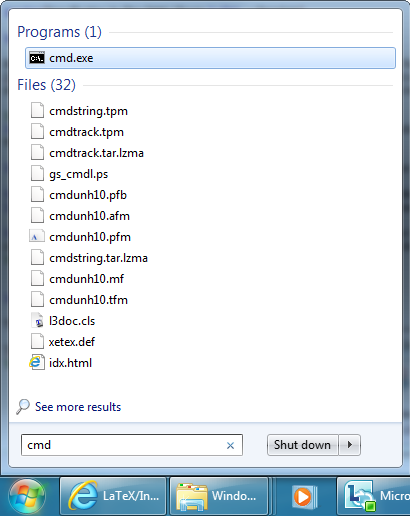
\includegraphics[scale=0.75]{TAMUthesis_CMD_windows.png}
\caption[Open CMD (Command Line Interface) under Windows]{Open CMD (Command Line Interface) under Windows
[Open the data/chapterI.tex file to search for the implementation of this figure, as you can
see that, to precisely control the position of the figure is not as straightforward as that in
Office Word.]}

\label{fig:CMD_1}

\end{figure}

\section{Figure Titles}

Some text here

\section{Continued Figures}
It's not recommended to use continued figures in this \LaTeX ~ document since figure/table numbering increases automatically. But if you would like to use it, refer to Figure \ref{fig:CMD_windows_cd_compile} for how Continued Figure works.

\begin{figure}[ht]
\centering
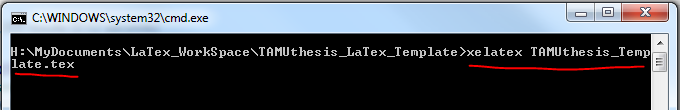
\includegraphics[scale=0.75]{TAMUthesis_CMD_windows_compile.png}
\caption{Compile .tex File}

\label{fig:CMD_windows_cd_compile}

\end{figure}
\cleardoublepage


\begin{figure}[ht]
\ContinuedFloat
\captionsetup{list=off, format=cont}
\centering
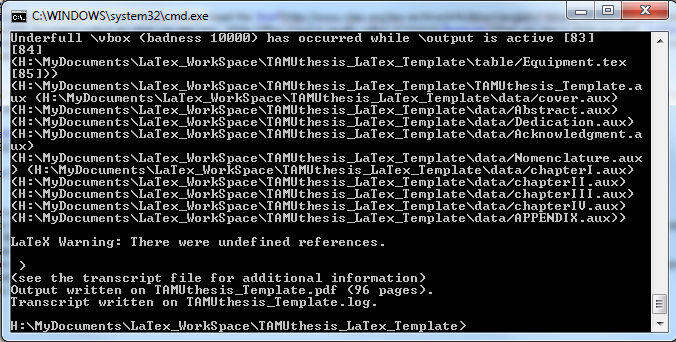
\includegraphics[scale=0.75]{TAMUthesis_CMD_windows_compile2.png}
\caption{[Example usage for Figure continued. Please don't display text for continued figures. This is just an example.]}

\label{fig:CMD_windows_cd_compile_continued}

\end{figure}


\section{Table Placement, Size and Table Title}


\begin{table}[!htbp]
\captionsetup{justification=centering}

\caption{Results from Experimental and Control Runs \label{table:control_runs}}

\begin{tabular}{|c|c|c|c|c|}
\hline
Species & Experiment 1 & Experiment 2 & Control 1 & Control 2\\
\hline
Cow & + & - & - & +\\
\hline
Brown Horse & - & + & - & -\\
\hline
Gray Cow &  &  &  & \\
\hline
White House & - & + & + & -\\
\hline
Tan Cow & + & - & - & +\\
\hline

\end{tabular}
\end{table}

 \cleardoublepage

 \begin{table}[!htbp]
 \ContinuedFloat
\captionsetup{list=off, format=cont}

 \label{table:control_runs_continued}
 
 \caption{} 

\begin{tabular}{|c|c|c|c|c|}
\hline
Species & Experiment 1 & Experiment 2 & Control 1 & Control 2\\
\hline
White Cow & + & - & - & +\\
\hline
Spotted Pig & + & + & + & -\\
\hline
White Pig & + & - & - & - \\
\hline
Brown Pig &  & + & + & -\\
\hline
Gray Pig & + & - & - & +\\
\hline
Black Pig & + & - & - & +\\
\hline

\end{tabular}
\end{table}



\section{Equations}

The following format is recommended to be used to display equations. The equation can be referred as Equ. \ref{Equ.2.1} and Equ. \ref{Equ.2.2}. 


\begin{equation} \label{Equ.2.1}
y'=y\cdot\cos{(a)}+x\cdot\sin{(a)}
\end{equation}

\begin{equation} \label{Equ.2.2}
e^{ja}=x\cdot\cos{(a)}-y\cdot\sin{(a)}
\end{equation}

Some sample equations are below


\begin{align}
V' &=e^{(ja)}\times V \label{Equ.3.3}\\
&=[\cos(a) + j \times \sin(a)] \times (x+j \times y) \label{Equ.3.4}\\
&=x \cdot \cos(a) - y\cdot \sin(a) + j \cdot [x \cdot \sin(a) + y \cdot     \cos(a)] \label{Equ.3.5}
\end{align}


\begin{equation}
\label{equ:matrix}
V=
\begin{bmatrix}
x'\\
y'\\
\end{bmatrix}=
\begin{bmatrix}
x \cdot \cos(a) - y \cdot \sin(a)\\
y \cdot \cos(a) + x \cdot \sin(a)\\
\end{bmatrix}
\end{equation}
Equ.\ref{equ:matrix} could be re-arranged as \ref{equ: 2.7} and  \ref{equ: 2.8}.

\begin{equation} 
\label{equ: 2.7}
x'=\cos(a) \cdot[x-y\cdot\tan(a)]
\end{equation}

\begin{equation} 
\label{equ: 2.8}
y'=\cos(a) \cdot [y+x \cdot \tan(a)]
\end{equation}



\begin{gather} 
x_{i+1}=\cos(a_i) \cdot [x_i-y_i \cdot 2^{-i} \cdot d_i] \label{Equ. 3.9}\\
y_{i+1}=\cos(a_i) \cdot [y_i+x_i \cdot 2^{-i} \cdot d_i] \label{Equ. 3.10}\\
\cos(\alpha)=\dfrac{1}{\sqrt [2]{1+{\tan(\alpha)}^2}}
 \label{Equ. 3.11} \\
K_i=\cos(\arctan(2^{-i}))= \dfrac{1}{\sqrt [2]{1+\tan(\arctan(2^{-   i}))}}=\dfrac{1}{\sqrt[2]{1+2^{-2i}}}
\label{Equ. 3.12}\\
\intertext{The product of $K_i$  represents the so-called $K$ factor (Equ. \ref{equ: 3.13})}
K=\prod K_i=\prod_{i=0}^{n-1} \dfrac{1}{\sqrt{1+2^{-2i}}}
\label{equ: 3.13}
\end{gather}


\section{Equation Vertical Spacing}

Test section for TOC display

\section{Other Information in this Document}
Test section for TOC display

\section{Another Test Section}
Test section for TOC display

\section{Another Test Section 3}
The section title is to test the toc only, no other purpose.

\section{Another Test Section 4}
Test section for TOC display

\section{Another Test Section 5 \& 6}
Test section for TOC display}







 





 

 
 

